\documentclass[10pt,a4paper]{article}
\usepackage[utf8]{inputenc}
\usepackage[russian]{babel}
\usepackage[OT1]{fontenc}
\usepackage{amsmath}
\usepackage{amsfonts}
\usepackage{amssymb}
\usepackage{amsthm}
\usepackage{makeidx}
\usepackage{graphicx}
\usepackage{tikz}
\usepackage{algorithm}
\usepackage{algorithmicx}
\usepackage{graphicx}
\usepackage{algpseudocode}
\usepackage{caption}
\usepackage{subcaption}

\usepackage{float}
\floatstyle{boxed}
\restylefloat{figure}

\author{Максим Борисяк}
\title{Дипломная работа}
\makeindex

\newtheorem{defen}{Определение}
\newtheorem{example}{Пример}
\newtheorem{theorem}{Теорема}
%\newtheorem{proof}{Доказательство}

\newcommand{\stock}{\text{STOCK}}
\newcommand{\source}{\text{SOURCE}}
\newcommand{\initial}{\text{INITIAL}}
\newcommand{\nontrivial}{\text{NON-TRIVIAL}}
\newcommand{\map}{\text{MAP}}

\newcommand{\FA}{F\!A}

%\textheight = 720pt
%\textwidth = 500pt

%\hoffset = -25mm
%\voffset = -30mm

\makeindex

\begin{document}

\maketitle

\section{Введение \textbf{*** Need review ***}}
В последние годы во многих областях науки, таких как, например, бионформатика или эксперементальная физика,
требуется обрабатывать все большее и большее количество данных.
В качестве примера можно привести Большой Адронный Коллайдер (БАК). 
В результате одного эксперимента поток 'сырых' данных с детектора \textit{ALICE} может превышать 1 гигабайт в секунду \textbf{[???]}.

Для обработки больших объемов данных используются распределенные вычислительные системы, мощности которых могут достигать пентафлопов.
Так для обработки данных БАК используется сложная распределенная система \textit{LHC Computing Grid}.
Такие мощности достигаются за счет громадного количества вычислительных узлов. Например, суперкомпьтер Sequoia мощностью более 1 пентафлопа
имеет более миллиона ядер \textbf{[???]}.

Однако с ростом объемов данных, и, как следствие, с ростом необходимых вычислительных ресурсов растет сложность задач эффективной обработки.
Известно, что принципы, лежащие в основе эффективных алгоритмов, могут существенно усложняться при переходе к параллельным вычислениям
и даже при изменении изменении масштабов вычислительных систем.

Другой проблемой становится сложность создания самих распределенных алгоритмов,
так как многие из них теряют наглядность из-за реализации большого количества технических аспектов, которые необходимо учитывать при их разработке.
Более того, некоторые распределенные системы не имеют четких границ, так как задействованные в ней участники могут постоянно меняться,
что дополнительно усложняет контроль за вычислениями.
Так для ускорения обработки результатов БАК был задействован проект \textit{LHC@home} \textbf{[???]}, помочь которому мог любой желающий путем предоставления части
вычислительной мощности собственного компьютера.

Одним из решений описанных выше проблем стала концепция \textit{потоков данных} (\textit{dataflow}).
Под потоком данных обычно понимают модель представления алгоритмов.
Описание вычислительного процесса в такой концепции, обычно, представляет из себя следующие элементы:
\begin{itemize}
  \item набор атомарных исполнителей-функций, реализованный вне концепции потоков данных, например, в виде программ или динамических библиотек;
  \item описание зависимостей между исполнителями --- результат работы одних исполнителей передается на вход (в качестве аргументов) другим;
  \item описание стратегии поведения потока данных;
  \item иерархичность --- иногда целый поток данных может быть представлен в виде одного исполнителя внутри другого потока данных.
\end{itemize}
Иными словами, поток данных представляется в виде наборов исполнителей, каждый из которых выполняет некое преобразование поступивших ему на вход данных,
соединенных каналам передачи данных.

Концепция потоков данных обладает важным приемуществом --- она полностью изолирует создателя алгоритма от необходимости описывать многие
технические аспекты вычислений. В этом они родственны декларативным языкам программирования, в которых программы выглядят как наборы определений или описаний зависимостей.
В частности, некоторые потоки данных можно без потери структуры преобразовать к программе, например, на языке Haskell \textbf{[???]}.

Другим приемуществом описания вычислительных процессов в виде потоков данных являются широкие возможности для автоматического
распределения ресурсов при запуске потока данных в распределенных средах, а также для предварительного анализа необходимых ресурсов для эффективного запуска.
Эти свойства являются крайне востребованными для научных вычислений, так как объемы вычислений явно требуют больших ресурсов недостижимых на систамах с одним потоком выполнения.
Как в примере c проектом \textit{LHC@home} потоки данных также хорошо описывают вычисления в динамических распределенных средах.
Возможность предварительной оценки требуемых ресурсов важна для эффективной утилизации мощностей суперкомпьютеров,
вычислительные способности которых могут заметно превосходить требуемые ресурсы. Так задаче получения таких оценок посвящена данная работа.

Родственной к потокам данных является концепция потоков управления (controlflow), основное отличие которых от потоков данных в том, что связи между исполнителями
означают передачу управления, и часто исполнители имеют доступ к общему хранилищу данных. Программы в терминах потоков управления имеют явно указанные
участки параллельного выполнения, создания и слияния параллельных ветвей.

Эти две концепции объединяют под названием поток работ (workflow).
Среди достоинств концепции потока работ следует выделить следующие:
\begin{itemize}
  \item изолированность программы, сценария или схемы от технических особенностей среди выполнения;
  \item наглядность программ --- чаще всего поток работ можно представить в графической нотации близкой к блок-схемам;
  \item простота создания программ --- создание программ, особенно в графичекой нотации, не требует специальных знаний из области информатики,
        что позволяет, например, физикам-эксперементаторам не тратить большое количество времени на изучение новых языков или сред обработки результатов.
\end{itemize}

В отличии от потоков упраления потоки данных, как уже было упомянуто, ориентированны на научные вычисления.
Среди особенностей можно выделить следующие:
\begin{itemize}
  \item работа в распределенных средах сложной динамичной структуры, ресурсы которой могут быть заранее неизвестны;
  \item высокая отказоустойчивость,
  \item работа с большим объемом данных.
\end{itemize}
Заметим, что среды построения и запуска потоков данных значительно отличаются по внутренним механизмам от
аналогичных сред для потоков управления из-за перечисленных выше отличий в концепциях.

Также стоит отметить, что потоки данных имеют
много общего с \textit{сетями процессов Кана} (\textit{Kahn Process Networks}), сходства и различия с которыми будет рассмотренно ниже.

Отметим также растущую популярность концепции потоков данных в научных кругах --- так в описанном выше примере с БАК,
для обработки результатов используются потоки данных или близкие к ним концепции \textbf{[???]}.

\subsection{Мотивация \textbf{*** Need review ***}}
В данной работе рассматривается модель потоков данных, которая, по мнению автора, предоставляет наиболее
естественное описание программ для научных рассчетов в концепции потоков данных.
Также рассматриваемая модель близка к моделям существующих и активно используемых сред для построения и запуска потоков данных.

В данной работе следует выделить несколько задач:
\begin{itemize}
  \item построение формальной модели потока данных;
  \item анализ потока данных на наличие ошибок;
  \item оценка ресурсов и стратегий, требуемых для эффективного запуска потока данных в распределенных средах.
\end{itemize}

Главные алгоритмы были реализованны в виде модуля языка Python для возможности
использования в интерактивном интерпретаторе для языка Python.

\subsection{Обзор существующих моделей представления потоков данных \textbf{*** Need review ***}}
Среди моделей представления потоков данных следует выделить следующие:
\begin{itemize}
  \item программы на высокоуровневых языках программирования;
  \item графы;
  \item сети Петри;
  \item сети процессов Кана.
\end{itemize}

Как уже было сказано, концепция сетей процессов Кана имеет некие отличия от рассматриваемой в этой работе концепции потоков данных,
однако определение потоков данных может варьироваться и обозначает скорее направление в представлении алгоритмов обработки,
поэтому можно считать сети процессов Кана, если не одной из моделей представления потоков данных, то как минимум родственной моделью,
и следовательно, заслуживающей рассмотрения как минимум для демонстрации возможных подходов.

\subsubsection{Программы на высокоуровневых языках программирования}
Любой вычислительный процесс можно наглядно описать в терминах современных языков программирования при дожном уровне абстракции от технических особенностей среды выполнения.
Наиболее подходящими языками для описания потоков данных являются скриптовые языки, например, Python, либо декларативные языки, например, Haskell или Erlang.
Декларативная парадигма, как уже было сказано, достаточно близка концепции потоков данных, однако порой декларативные языки слишком строги для описания потоков данных.

Основной проблемой такого подхода является недостаточная наглядность для людей не знакомых с конкретным языком программирования и требует знания возможных тонкостей этого языка.
Более того, обычно визуальное преставление является более наглядным для человека, чем текстуальное. Этим можно объяснить меньшую популярность такого подхода.

В качестве примера системы, использующей языки программирования как представление потока данных, можно привести систему \textit{GridAnd} \textbf{[???]}.

\subsubsection{Графы}
Графы являются самой популярной моделью потоков данных.
Главным достоиством является возможность интуитивно понятного визуального представления графов, которое не требует специальных знаний в области информатики.

Другим достоинством графов как модели представления потока данных является возможность построения иерархичных потоков данных, где один поток данных,
представляется в виде вершины в потоке более высокого уровня, тем самым реализуя принципы модульности и абстракции.

Особо стоит выделить хорошо изученные свойства графов и множетво алгоритмов для их анализа, а так же выразительную силу графов.
Например, в данной работе с помощью графов описываются сами потоки данных, качественно поведение каждого блока (в виде конечного автомата),
поведение блока во время запуска потока данных (также в виде автомата).

\subsubsection{Сети Петри}
Другой популярной концепцией представления потоков данных являются сети Петри, которые можно считать развитием идеи графов.
Как и в случае с графами, сети Петри можно наглядно представить используя визуальные средства.

Также доступен широкий набор средств для анализа сетей Петри. Кроме того, в сетях Петри явно присутствуют элементы паралелизма,
хотя сети Петри лучше подходят для описания потоков управления (чем возможно объсняется их популярность в системах построения потоков управления),
нежели потоков данных, так как переход так называемых маркеров от одного узла к другому означает
скорее передачу управления, нежели передачу данных. Однако представление потоков данных в виде сетей Петри также возможно.

\subsubsection{Сети процессов Кана}
Сети процессов Кана используются для описания потоков данных ориентированных на потоковую обработку, в отличии от рассматриваемой в этой работе
модели, где данные подаются на вход поэлементно или одной 'порцией'.
Формально в этой концепции каждый процесс (исполнитель) представляется функцией, которая преобразует входящие потоки данных целиком, и лишь
в частном случае это эквивалентно поэлементной обработке.
В таких случаях мы получим концепцию близкую к концепции потоков данных. Однако в сетях процессов Кана для разрешения возможных неопределенностей в 
поведении процессов накладываются ограничения на функции, которыми представляется процесс, вводятся правила поглощения и испускания данных; в концепции потоков данных вместо наложения ограничений на функции стараются анализировать саму схему потока данных, которая, так как не является потоковой, сама по себе может не допускать потенциальных неопределенностей \textbf{[???]}.

Стоит также отметить, что сети процессов Кана, аналогично потокам данных,
могут быть естественно представленны с помощью декларативных языков программирования.
Например, используя функции преобразующие бесконечные списках в языке Haskell, можно добиться точного соответствия формального определению сетей процессов Кана. 

\subsection{Неформальное описание модели \textbf{*** Need review ***}}

В качестве основы для построения модели были взяты основные принципы работы популярных сред построения и запуска потоков данных.
Сам поток данных представляется в виде ориетированного графа, вершинами которого являются блоки.
Блоки реализуют некий алгоритм преобразования данных и в зависимости от способа создания этого алгоритма деляться на два типа:
\begin{itemize}
  \item атомарные --- встроенные в систему построения и запуска потоков данных в виде внутренних подпрограмм;
  \item составные --- блок, который сам представляется в виде потока данных и является вложенным потоком данных.
\end{itemize}
У каждого блока (кроме специальных или 'фиктивных') существуют наборы входных и выходных портов. Входные порты в некотором смысле являются 'аргументами' блока ---
по ним передаются данные для преобразования. Выходные порты имеют смысл результата выполнения преобразования --- по ним данные передаются для дальнейшей обработки.
Каждый порт обычно обладает определенным смыслом, который определяется алгоритмом преобразования.

Ребро графа потока данных соединяет выходной порт одного блок с входным портом другого блока, задавая тем самым, последовательность обработки данных.
Ребра можно также рассматривать как FIFO-каналы, передача по которым ради простоты будем считать мгновенной.

Естественно, что работа потока данных зависит от внутренних состояний программ его блоков. В данной работе алгоритмы блоков заменяются на конечные автоматы Мили,
описывающие зависимости наборов выходных данных от входных. Таким образом мы получаем качественное описание работы блоков, что существенно упрощает
задачу анализа, освобождая от необходимости описывать анализ алгоритмов блоков, который выходит за рамки рассматриваемых вопросов.

Стоит отметить, что обычно данные имеют тип, однако рассмотрение типов данных приводит к усложнению модели,
не приводя при этом ни к каким дополнительным результатам.

\subsection{Базовые понятия и определения \textbf{*** Need review ***}}
В данном разделе будут введены базовые понятия, используемые в данной работе, в том числе,
понятия атомарного блока, составного блока, потока данных, автомата Мили соответствующего блоку и так далее.

Основной единицей потока данных является атомарный блок.
\begin{defen}
  \textbf{Шаблоном атомарного блока} $s$ назовем кортеж имеющий два не пересекающихся набора портов: \textit{входной} и \textit{выходной}.
  $s = (\FA, I, O)$, где:
  \begin{itemize}
    \item $I = \{b^I_i \vert i = \overline{1, N_I}, N_I \in \mathbb{N}\}$ --- конечное множество уникальных входных портов;
    \item $O = \{b^O_i \vert i = \overline{1, N_O}, N_O \in \mathbb{N}\}$ --- конечное множество уникальных выходных портов;
    \item $\FA$ --- конечный автомат Мили, смысл и структура которого будет обсуждаться в дальнейшем.
  \end{itemize}
\end{defen}
Сразу заметим, что не любая тройка $(\FA, I, O)$ является шаблоном атомарного блока, так как $\FA$ должен
соответствовать множествам $I$ и $O$.

Стоит отметить, что природа множеств $O$ и $I$ совершенно не важна, например, они могут быть просто множеством чисел: $I, O = \{i \in \overline{1, \dots, N_{I, O}}\}$,
на практике часто используют строки для именования портов, так как порты могут существенно различаться по смыслу, а их именование помогает избежать путаницы.
Последний подход используется в рисунках.

\begin{defen}
  \textbf{Атомарным блоком} $b = (id, s, state)$, где:
  \begin{itemize}
    \item $id$ --- уникальный для всех блоков идентификатор;
    \item $s$ --- шаблон атомарного блока;
    \item $state \in S$, где $S$ множество состояний $\FA_s$ --- текущее состояние атомарного блока.
  \end{itemize}
\end{defen}

Идентификатор $id$ введен из-за следующих соображений: в потоке данных некие блоки могут описываться одним и тем же шаблоном, находиться в одном и том же состоянии,
но все равно будут являться различными блоками, в частности, могут перейти в различные состояния в следующие моменты времени либо могут иметь в потоке данных разный смысл и,
соответственно, иметь различные соединения с другими блоками.

В реальных системах для построения и запуска потока данных шаблон атомарного блока представляется в виде подпрограммы или модуля
(функции, класса некого объектно-ориентированного языка программирования, динамической библиотеки), который используя данные некого набора своих входных портов,
вычисляет и записывает данные в свои выходные порты. В таком случае, атомарный блок представляется в виде набора внутренних переменных,
либо (что тоже самое) в виде экземпляра класса объектно-ориентированного языка программирования соответствующего шаблону.
В такой интерпретации некую вычислимую функцию $f(x_1, x_2, \dots, x_n)$ можно представить в виде шаблона блока $b_f$
с входными портами $x_1, x_2, \dots, x_n$ и одним выходным портом $F$, который при получении данных со всех входных портов
выписывает значения функции $f(x_1, x_2, \dots, x_n)$ в порт $F$.

На рисунке \ref{map} схематично изображен шаблон блока \textit{Loop}, для которого $inputs(Loop) = \{xs, f\}$, $outputs(Loop) = \{fs, x\}$.

\begin{figure}[H]
  \centering

  \begin{subfigure}[b]{0.2\textwidth}
    \centering
    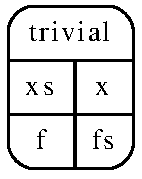
\includegraphics[width=\textwidth]{map_cg.pdf}
    \caption{Схема шаблона \textit{Loop}}
    \label{map:connection}
  \end{subfigure}
  ~
  \begin{subfigure}[b]{0.7\textwidth}
    \centering
    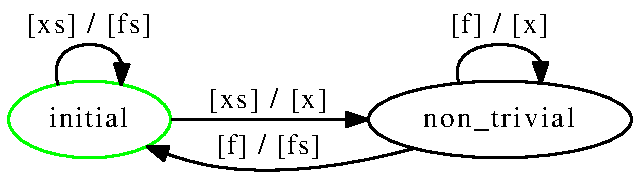
\includegraphics[width=\textwidth]{map_fa.pdf}
    \caption{Автомат Мили шаблона \textit{Loop}}
    \label{map:fa}
  \end{subfigure}
  
  \caption{Схематичное изображение шаблона блока \textit{Loop} (a) и соответствующего ему конечного автомата Мили (b).}
  \label{map}
\end{figure}

Основной структурой для построения схемы потока данных является составной блок.

\begin{defen}
 \textbf{Шаблоном составного блока} будем называть кортеж $c = (B, E, I, O)$, где:
 \begin{itemize}
    \item $B$ - конечное множество блоков (сразу заметим, что блоком может являться и составной блок, определенный ниже).
    \item $E$ - множество ребер вида $e_b = (b_1, b^O_{1}, b_2, b^I_{2})$, $b_1, b_2 \in B$, $b^O_{1} \in outputs(b_1), b^I_{2} \in inputs(b)$,
                либо вида $e_I = (c^I, b, b^I)$, $e_O = (b, b^O, c^O)$, где $b \in B$, $b^I \in inputs(b)$, $b^O \in outputs(b)$, $c^O \in O$, $c^I \in I$.
                Множества ребер $e_b$ будем обозначать как $E^B$, $e_I$ и $e_O$ как $E^I$ и $E^O$ соответственно.
    \item $I$, $O$ - конечные наборы входных и выходных портов (по аналогии с атомарным блоком).
  \end{itemize}
\end{defen}

В дальнейшем в выражениях вида $I_c$ или $O_c$ нижний индекс будет указывать на схему блока, которому принажлежат эти множества.

Для анализа внутренней структуры удобно рассматривать иное представление шаблона составного блока $c$, добавляя фиктивные блоки $\stock$, $I_{\stock} = O_{\stock} = O_c$,
  и $\source$, $I_{\source} = O_{\source} = I_c$:
$$\hat{E}^I = \{(\source, \source^O, b, b^I) \vert (\source^O, b, b^I) \in E^I\}$$
$$\hat{E}^O = \{ (b, b^O, \stock, \stock^I) \vert (b, b^O, \stock) \in E^O \}$$
$$\hat{c} = (B \cup \{\stock, \source\}, E^B \cup \hat{E}^I \cup \hat{E}^O)$$
В этом случае шаблон составного блока $\hat{c}$ описывается графом с ребрами вида $(u, u^O, v, v^I)$,
а входными и выходными портами всего шаблона считаются входные и выходные порты блоков $\source$ и $\stock$.
На рисунке \ref{example} изображен примеры шаблонов составных блоков во втрой интерпретации.

\begin{defen}
  \textbf{Составным блоком} будем называть $b = (id, c = (B, E, I, O), state)$, где
  \begin{itemize}
    \item $id$ --- уникальный идентификатор;
    \item $c$ --- шаблон составного блока;
    \item $state \in \Sigma \times 2^E = \prod S(B) \times 2^E$ - текущие состояние составного блока, включающее
          состояние каждого блока (подпространство $\Sigma = \prod S(B)$), активную волну ($\omega \in \Omega = 2^E$).
  \end{itemize}
\end{defen}

\begin{figure}[H]
  \centering
  \begin{subfigure}[b]{0.3\textwidth}
    \centering
    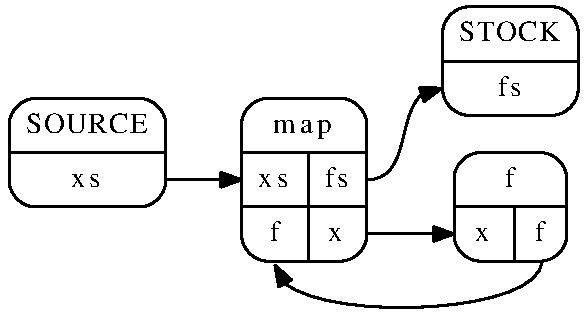
\includegraphics[width=\textwidth]{example_cg.pdf}
    \caption{Шаблон составного блока}
    \label{example:composite}
  \end{subfigure}
  ~
  \begin{subfigure}[b]{1.0\textwidth}
    \centering
    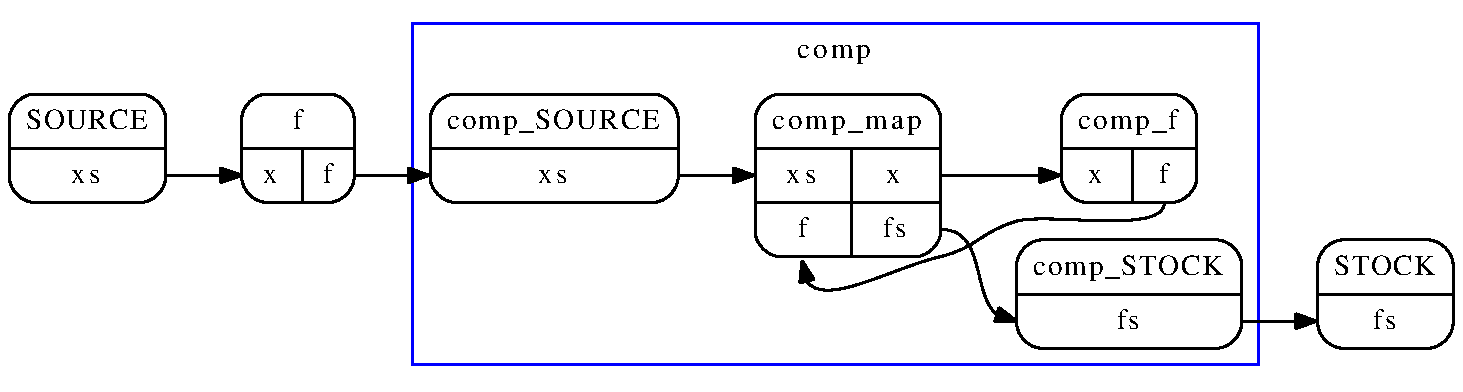
\includegraphics[width=\textwidth]{cc_cg.pdf}
    \caption{Шаблон супер-составного блока. Внутри рамки показана структура шаблона внутреннего блока.}
    \label{example:supercomposite}
  \end{subfigure}
  
  \caption{ Примеры графов составного и супер-составного блока.}
  \label{example}
\end{figure}

Заметим, что составной блок (в исходной интерпретации) внешне не отличим от атомарного блока.
Поэтому под понятием блока мы будем подразумевать либо атомарный блок, либо составной блок,
различая их только в том случае, когда речь заходит о их внутреннем строении. Составной блок может включать в себя другие составные блоки.
На рисунке \ref{example:supercomposite} показан пример составного блока, включающего другой составной блок, иными словами супер-составного блока.
На практике свойство вложенности реализует принцип модульности программ --- модулем в нашем случае будет шаблон составного блока.
Бессмысленно рассматривать случаи, в которых структура составного блока бесконечна в глубину, например,
в случае когда шаблон составного блок содержит содержит блок того же шаблона. Поэтому в дальнейшем, мы будем рассматривать только составные блоки конечной глубины.

Заметим, что составным блоком можно описать любую программу, имея в распоряжении необходимые примитивы --- шаблоны атомарных блоков,
реализующие Тьюринг-полную систему операций. Доказательства этого факта выходит за задачи данной работы и может быть найдено, например, в работе \textbf{[???]}.
Из-за достаточной выразительности составного блока, схему потока данных мы определим просто как схему некого составного блока.

Теперь неформально поясним схему работы составного блока и смысл его структуры.
В общепринятых определениях потока данных ребра графа шаблона составного блока обозначают зависимость по данным, то есть ребро $e = (u, u^O, v, v^I)$ представляет собой
\textit{FIFO}-канал соединения между портами блоков и
можно словесно интерпретировать следующим образом: блок $v$ в качестве данных из входного порта $v^I$ должен использовать данные выходного порта $u^O$ блока $u$ при их наличии.
Блок $u$ после завершения своей работы может "испустить данные по порту $u^O$", которые мгновенно "переносятся" на все ребра из $u^O$ блока $u$,
если эти ребра свободны.
Когда блоку $v$ требуются данные из порта $v^I$, данные с ребра $e$ мгновенно "переносятся" в соответствующий порт блока. В этом и есть смысле подпространства $\Omega = 2^E$
в определении состояния составного блока --- \textit{активной волной} $\omega$ мы назовем множество ребер, которые содержат на данный момент данные.

Однако такая схема работы составного блока порождает множество неопределенностей в работе некоторых составных блоков, например, неопределенность выбора ребра для "поглощения" данных из определенного порта (состояние гонки).
Неопределенности подобного рода мы будем рассматривать как ошибки, обнаружению которых посвящена часть данной работы. Такого рода неодназначности, особенно в реальных системах,
то есть в условиях неопределенного времени вычислений блоков и их параллельного выполнения, может привести к совершенно иному ходу потока данных, нежели было задумано автором потока данных.
Поэтому наличие подобного рода неопределенностей (состояний гонки) говорит скорее о неправильном построении схемы потока данных, чем о некой задумке автора потока данных.
Более подробно и строго об неоднозначностях в поведении потока данных будет идти речь ниже.
Стоит заметить, что подобного рода неоднозначности возникают и в процессе определения сетей процессов Кана,
которые решаются наложением условий на правила поглощения и испускания, а также на класс функции процесса.
Мы же пойдем другим путем, накладывая ограничения лишь на граф шаблона потока данных, оставляя подпрограммы и правила поглощения каждого шаблона блока без ограничений.
В нашем случае правила поглощения состоят в том, что формально блок может поглотить любые доступные данные из любых портов по любым ребрам,
но будем расценивать любые возможные неоднозначности как ошибку построения потока данных.

Выше были рассмотрены определения и термины, которые с той или иной точностью присутствуют практически во всех моделях потока данных.
В данной работе мы абстрагируемся от данных, а значит нас интересуют только возможные зависимости наборов входных портов от набора выходных портов,
иными словами только качественное поведение блоков. Оказывается, конечный автомат Мили хорошо подходит для описания качественного поведения блоков.
Заметим, что в данной работе используется не стандартное определение автомата Мили, а его недетерминированные аналог.
Дадим теперь строгое определение конечного автомата Мили.

\begin{defen}
  \textbf{Конечный автомат Мили} --- кортеж $\FA = (S, s_0, \Sigma, \Lambda, E)$, где:
  \begin{itemize}
    \item $S$ --- конечное множество состояний;
    \item $s_0 \in S$ --- начальное состояние;
    \item $\Sigma$ --- входной алфавит;
    \item $\Lambda$ -- выходной алфавит;
    \item $E \subseteq S \times \Sigma \times \Lambda \times S$ --- отношение возможных переходов.
  \end{itemize}
\end{defen}

Для удобства будем рассматривать функцию конечного автомата Мили $\FA = (S, \cdot, \Sigma, \Lambda, E)$:
$\FA(p, \lambda) = \{(\sigma, q, \lambda') \vert (p, \lambda', \sigma, q) \in E, \lambda' \subseteq \lambda\}$.
Стоит обратить внимание на нестандартную форму данной функции. Далее символами в алфавитах $\Sigma$ и $\Lambda$ будут множества, поэтому функция по текущему состоянию и входному множеству возвращает множество троек вида:
выходной символ-множество, новое состояние и поглощенное множество.

Конечный автомат Мили выполняет преобразование последовательности входных символов из алфавита $\Sigma$ в последовательность символов в алфавите $\Lambda$.
Вернемся теперь к определению шаблона атомарного блока. В данной работе мы абстрагируемся от конкретного алгоритма преобразования входных данных в выходные
и преобразования внутреннего состояния блока. Вместо этого мы будем описывать лишь качественное поведение алгоритма автоматом Мили $\FA$, в котором входной алфавит
$\Sigma = 2^I \setminus \varnothing$ (запрещается запуск по пустому набору входных портов),
а выходной алфавит $\Lambda = 2^O$, иными словами ребро $e = (u, is, os, v)$ автомата $\FA$ описывает возможный переход из состояния $u$ в состояние $v$,
при считывании данных из портов $is$ и выписывании данных в порты $os$ (именно поэтому функция $\FA$ имеет странный на первый взгляд вид).
На практике подпрограмма реализующая логику атомарного блока может иметь значительное количество внутренних состояний,
однако, для наших целей важны лишь группы таких внутренних состояний, которые описывают возможное поведение на определенном наборе данных из входных портов.
Более того практически во всех системах построения и запуска потока данных подпрограмма описывающая блок имеет детерминированное поведение.
Неизбежный недетерминизм в автомате Мили, описывающий блок, возникает из-за исключения из рассмотрения самих данных,
так как при разных значениях на одном и том же наборе портов из одного состояния, блок может перейти в различные конечные состояние,
даже выписав при этом данные в один и тот же набор портов.

\begin{example}
  На рисунке \ref{map:fa} изображен автомат Мили для шаблона атомарного блока $Loop$, описывающего цикл. Поясним эту схему.
  Изначально блок с шаблоном $Loop$ находиться в состоянии \textit{initial}.
  Далее он может считать из порта \textit{xs} начальные параметры цикла (например, некую коллекцию данных).
  Если условие выхода из цикла изначально выполнено (например, пустая коллекция), то блок переходит в прежнее состояние выписав в порт \textit{fs}.
  Иначе, блок отправляет данные по порту \textit{x} переходя в состояние \textit{non\_trivial}. В состоянии \textit{non\_trivial} блок имеет не тривиальное внутреннее состояние,
  например, остаток коллекции. В этот состоянии блок ожидает поступление преобразованных некой внешней функцией данных на порт \textit{f}.
  И в этом случае существует два варианта перехода, в зависимости от выполнения условия выхода из цикла:
  $(non\_trivial, \{f\}, \{x\}, non\_trivial)$ и $(non\_trivial, \{f\}, \{fs\}, trivial)$ для случаев продолжения цикла и выхода из него соответственно.
\end{example}

Конечный автомат Мили может быть также определен для составного блока. Единственное отличие от автомата Мили для атомарного блока состоит в том, что
зная все автоматы внутренних блоков, можно вычислить автомат составного блока как будет показано ниже.

\subsubsection{Алгоритм работы потока данных \textbf{***Need review***}}
Теперь опишем алгоритм вычисления потока данных, представленного в виде составного блока $c$ со схемой
$C = (\hat{B}_c = B_c \cup \{\source, \stock\}, \hat{E}_c= E_c \cup E^I_c \cup E^O_c)$ в представлении графа.
Мы будем рассматривать вычисление потока данных в предположении,
что время работы блока может быть абсолютно любым (но конечным) при любых условиях, что полностью соответствует реальным потокам данных.
В таком случае нас прежде всего будет интересовать всевозможные поведения потока данных с точки зрения относительных расположений времен запуска и завершения любого блока.
Введем модельное время $t \in \mathbb{Z}_+$.
Каждое множество, связанное с состоянием системы в момент времени $t$, снабдим верхним индексом, например, $\omega^t \in \Omega_c$.

\begin{defen}
  Определим некоторые вспомогательные функции.
  \begin{eqnarray*}
    O_v(\omega) & = & \{v^O \vert (v, v^O, \cdot, \cdot) \in \omega\}, \\
    I_v(\omega) & = & \{v^I \vert (\cdot, \cdot, v, v^I) \in \omega\}, \\
    \Delta_{O, v} & = & \{(v, v^O, \cdot, \cdot) \in E_c \vert v^O \in O\}, \\
    \Delta_{I, v} (\omega) & = & \{\tilde \omega_{I, v} \subseteq \omega \}, \; \forall \tilde \omega_I \forall v^I \in I \exists ! e \in \omega_I: e = (\cdot, \cdot, v, v^I)
  \end{eqnarray*}
\end{defen}
Последняя функция возвращает множество вариантов поглощения по набору входных портов $I$ блока $v$.

\begin{defen}
  Фронтом $\Psi_c (\omega, s)$ активной волны $\omega = \{(u, u^O, v, v^I)\} \in \Omega_c$ в состоянии $(s = (s_{u_1}, s_{u_2}, \dots, s_{u_m}), \omega, \cdot)$
  назовем подмножество блоков $\Psi_c (\omega, s) \subseteq B_c$, такое что:
  $$\Psi_c (\omega, s) = \{ v \in B \vert \FA_v(s_v, I_v(\omega)) \neq \varnothing\}$$
\end{defen}
Иными словами, фронт активной волны в заданном состоянии --- множество блоков, которые могут быть запущенны на следующем шаге.

\begin{defen}
  Семейство $\pi^t_v \in E_v, \; \FA_v = (\cdot, \cdot, E_v, \cdot)$ показывает текущий переход, который совершает блок $v$ в момент времени $t$.
\end{defen}
Заметим, что значение $\pi^t_v$ имеет смысл только для работающих на шаге $t$ блоков.

\begin{defen}
  Условием излучения назовем $\zeta(\omega^t, \omega^O) \Leftrightarrow (\omega^O \cap \omega^t = \varnothing)$.
  Также определим семейства $\zeta^t_v$:
  $$\zeta^t = \{ v \in B_c \vert zeta(\omega^t, \omega^O_v) \}$$
  $$\omega^O_v = \{ e \in E_c \vert e = (v, v^O, \cdot, \cdot), v^O \in O^t_v \}, \; (\cdot, O^t_v, \cdot, \cdot) \in \pi^t_v$$
\end{defen}
Условие излучение звучит довольно просто: блок может излучить, если все ребра соединенные с выходным набором портов свободны.

Пусть $\phi^t \subseteq \vartheta^t$ --- множество блоков, которые закончат работу после шага $t$. Для любого времени это множество может быть произвольным подмножеством $\vartheta^t$.
Однако для любого семейства этих множеств должно выполняться условие конечной работы блока: $\forall t \forall b \in \theta^t \exists \tau > t: b \in \phi^{\tau}$.

Так же для удобства введем обозначение для любого множества $A_c$ блоков из $B_c$ --- $A_c(v) \Leftrightarrow v \in A_c, v \in B_c$.

Теперь выпишем алгоритм преобразования потока данных в виде условий на переходы каждого блока из одного множества в другое.
В каждый момент времени блок $v$ может находиться в одном из трех состояний (множеств): свободен ($v \in \xi^t$), работает($v \in \theta^t$), заблокирован($v \in \chi^t$).
Время работы блоков задается $\phi^t \subseteq \vartheta^t$ --- множеством блоков, которые закончат работу после шага $t$. Для любого времени это множество может быть произвольным подмножеством $\vartheta^t$. Однако для любого семейства этих множеств должно выполняться условие конечной работы блока: $\forall t \forall b \in \theta^t \exists \tau > t: b \in \phi^{\tau}$.
Эти состояние взяты из реальных систем запуска потоков данных и служат для интуитивного понимания модели. В дальнейшем, однако, мы избавимся от этих состояний.
Также введем семейства  --- переход автомата Мили блока, который совершает блок в текущий момент.

\begin{eqnarray}
  % Free and can not be launched => Free
  \xi^t(v) \wedge \neg \Psi_c(\omega^t, s^t)(v) & \Rightarrow &
    \begin{cases}
      \xi^{t + 1}(v), \\
      s^{t + 1}_v = s^t_v, \\
      \omega^t_{I, v} = \omega^t_{O, v} = \varnothing
    \end{cases} \label{freetofree} \\
    % Free and can be launched => Work
  \xi^t(v) \wedge \Psi_c(\omega^t, s^t)(v) \wedge v \neq \stock & \Rightarrow &
    \begin{cases}
      \theta^{t + 1}(v), \\
      (\cdot, \cdot, I^t_v) \in \FA_v(s^{t}_v, I_v(\omega^t)), \\
      \pi^{t + 1}_v \in \{ (s^t_v, I^t_v, \cdot, s^{t + 1}_v) \in E_v\}, \\
      \omega^t_{I, v} \in \Delta_{I^t_v, v}(\omega^t), \\
      \omega^t_{O, v} = \varnothing
    \end{cases} \label{freetostart}
\end{eqnarray}

\begin{eqnarray}
  % Work and will not finish => Work
  \theta^t(v) \wedge \neg \phi^t(v) & \Rightarrow &
   \begin{cases}
     \theta^{t + 1}(v), \\
     s^{t + 1}_v = s^t_v, \\
     \pi^{t + 1}_v = \pi^t_v, \\
     \omega^t_{I, v} = \omega^t_{O, v} = \varnothing
   \end{cases} \label{worktowork} \\
   % Work, will finish and can be finished => Free
  \theta^t(v) \wedge \phi^t(v) \wedge \zeta^t(v) & \Rightarrow &
    \begin{cases}
      \xi^{t + 1}(v), \\
      (s^t_v, \cdot, O^t_v, s^{t + 1}_v) = \pi^t_v, \\
      \omega^t_{O, v} = \Delta_{O^t_v, v}, \\
      \omega^t_{I, v} = \varnothing
    \end{cases} \label{worktofree}\\
  % Work, will finish and can not be finished => Blocked
  \theta^t(v) \wedge \phi^t(v) \wedge \neg \zeta^t(v) & \Rightarrow &
    \begin{cases}
      \chi^{t + 1}(v),\\
      \pi^{t + 1}_v = \pi^t_v, \\
      \omega^t_{O, v} = \omega^t_{I, v} = \varnothing
    \end{cases} \label{worktoblock}
\end{eqnarray}

\begin{eqnarray}
  % Blocked and can release data => Free
  \chi^t(v) \wedge \zeta^t(v) & \Rightarrow &
    \begin{cases}
      \xi^{t + 1}(v), \\
      (s^t_v, \cdot, O^t_v, s^{t + 1}_v) = \pi^t_v, \\
      \omega^t_{O, v} = \Delta_{O^t_v, v}, \\
      \omega^t_{I, v} = \varnothing
    \end{cases} \label{blocktofree} \\
  % Blocked and can not release data => Blocked
  \chi^t(v) \wedge \neg \zeta^t(v) & \Rightarrow &
    \begin{cases}
      \chi^{t + 1}(v), \\
      s^{t + 1}_v = s^t_v, \\
      \pi^{t + 1}_v = \pi^{t}_v, \\
      \omega^t_{O, v} = \omega^t_{I, v} = \varnothing
    \end{cases} \label{blocktoblock}
\end{eqnarray}

\begin{eqnarray}
  \omega^{t + 1} & = & \omega^t \setminus (\cup_{v \in B_c} \omega^t_{I, v}) \cup (\cup_{v \in B_c} \omega^t_{O, v}) \label{newomega}, \\
  s^{t + 1} & = & (s^t_{v_1}, \dots, s^t_{v_m}) \label{newstate}
\end{eqnarray}

\begin{figure}
    \centering
    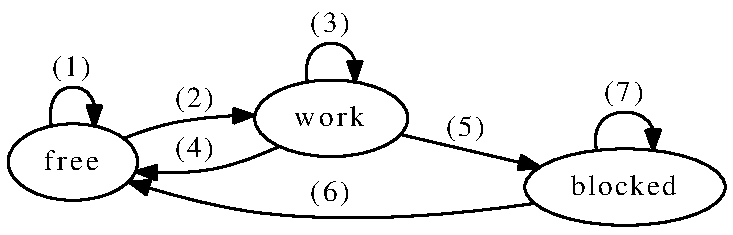
\includegraphics[width=\textwidth]{rules.pdf}
    \caption{Схема работы блока}
    \label{rules}
\end{figure}

Работу каждого блока можно схематично изобразить в виде автомата, см. рисунок \ref{rules}.

Поясним эти правила. Каждое правило \eqref{freetofree} --- \eqref{blocktoblock} описывает условие перехода в конечном автомате на рисунке \ref{rules}.

Правила \eqref{freetofree} и \eqref{freetostart} говорят о поведении свободного блока --- если блок может запуститься из его текущего состояния $s^t_v$
(то есть хватает данных на портах для какого-либо перехода), то он поглощает данные $\omega^t_{I, v}$ и
начинает некий переход $\pi^{t+1}_v$ из текущего состояния, иначе остается свободным дальше.

Тройка правил \eqref{worktowork}, \eqref{worktofree} и \eqref{worktoblock} описывают поведение работающего блока $v$. Если множество $\phi^t$ не содержит рассматриваемый блок,
он продолжает работу. Иначе, возможны два варианта: либо блок может завершиться и испустить данные $\zeta^t(v)$ (то есть ребра $\Delta_{O^t_v, v}$, связанные с
испускаемыми портами $O^t_v$, свободны), то блок благополучно завершает работу $\xi^{t + 1}(v)$ и испускает данные ($\omega^t_{O, v}$),
либо блок переходит в состояние блокировки до момента, когда требуемые ребра освободятся, которое описывается правилами \eqref{blocktofree} и \eqref{blocktoblock}.

Заметим, что мы специально различаем состояния блокировки и работы, хотя можно было бы считать, что заблокированный блок просто работает дополнительное время.
Состояние блокировки отличается тем, что блок в этом состоянии не требует вычислительных ресурсов, что будет важно в дальнейшем.

Заметим, что в правилах поведения потока данных сразу видны все неопределенности, о которых говорилось ранее --- перед запуском блока, определяется переход,
который будет совершать блок, вместе с набором поглощаемых портов и ребра с которых эти данные будут поглащены. Подробнее мы будем рассматривать эти неопределенности далее.

\subsubsection{Начало и завершение работы потока данных}
  Если рассматривать представление потока данных в виде графа, то начало и завершение потока данных связанно с дополнительными или 'фиктивными'
  блоками $\source$ и $\stock$: их задачи сформировать начальную и поглотить конечную активные волны, соответственно.
  Исходя из правил, можно записать начальные условия:
  \begin{eqnarray}
    \omega^0 & = & \varnothing, \\
    s^0_v & = & s_{0, v}, \forall v \in B_c, \\
    \theta^0 & = & \{\source\}, \\
    \xi^0 & = & B_c \setminus \{\source\}, \\
    \chi^0 & = & \varnothing, \\
    \omega^1 & \neq & \varnothing
  \end{eqnarray}
  
  Формирование начальной волны заложено в принципе работы блока $\source$.
  Так как блоки $\source$ и $\stock$ являются вспомогательными, то нет смысла рассматривать их автоматы Мили, так как атомат для блока $\source$ не может иметь ни одного перехода
  из-за отсутствия входных портов, а автомат для блока $\stock$ будет создавать дополнительные неопределенности при анализе потока данных.
  Будем считать, что работа этих блоков определяется следующим образом: $\source$ на первом шаге испускает некий непустой набор входных данных --- начальную активную волну;
  блок $\stock$ поглощает все данные на его портах, если никакие другие блоки больше не могут запуститься. Именно запуск блока $\stock$ мы будем считать завершением работы
  всего потока данных, иными словами, поток данных завершает работу на шаге $t = T_{end}$, если:
  \begin{equation}
    \theta^{T_{end}} = \varnothing \wedge \Psi_c(\omega^{T_end}, s^{T_end}) = \{\stock\}
    \label{end_of_workflow}
  \end{equation}
  Завершение работы потока данных связанно с понятием траектории запуска потока данных и более подробно будет рассмотренно ниже.

\section{Анализ модели \textbf{*** Need review ***}}
\subsection{Построение конечного автомата Мили по программе блока \textbf{***Need review***}}
Введенная выше модель оперирует с упрощенными описаниями алгоритмов блоков --- каждый алгоритм заменяется на описывающий его качественное поведение автомат Мили.
Каждое состояние конечного автомата соответствует группам внутренних состояний алгоритма блока. Разбиение на группы можно производить с большой свободой.
Сразу же заметим, для дальнейшего анализа будет полезно выделить особое состояние конечного автомата Мили для блока --- начальное состояние (далее будет обозначаться словом $\initial$), соответствующее начальным значениям внутренних переменных. Это состояние обладает значительной особенностью, а именно, блок находящийся в нем, фактически
не занимает ресурсов памяти вычислительного узла, поэтому может быть просто перенесен на другой вычислительный узел без дополнительных затрат
на копирование внутреннего состояния с одного вычислительного узла на другой. Процедуры перемещения состояния алгоритма блока на другой
вычислительный узел играют важную роль в управлении запуском потока данных в распределенной среде (более подробно запуск потока данных в распределенной среде будет рассмотрен ниже), так как ожидающий данных блок будет заблокирован (или по, крайней мере, может быть дополнительно ограничен в вычислительных ресурсах),
если на вычислительном узле на момент поступления данных первому блоку выполняется алгоритм другого блока, но может быть инициализирован на свободном
(если таковые имеются) вычислительном узле, если блок находится в начальном состоянии.

Построение автомата Мили для алгоритма блока --- неодназначная задача, требующая понимания качественного поведения алгоритма, а значит участия человека. В данной работе подробно не рассматриваются алгоритмы (которые, по мнению автора, будут бесполезны на практике в силу огромных вычислительных затрат) и методики построения атоматов Мили для алгоритмов блоков. Ограничемся лишь рассмотрение показательного примера с шаблоном блока \textit{For-Loop}. В зависимости от реализации, блок \textit{For-Loop} принимает на вход данные о количестве необходимых операций, для опреденности будем рассматривать шаблон блока, реализующий аналог функции \textit{map} популярной в функциональных языках программирования,
которая поэлементно применяет переданную ей в качестве аргумента функцию к списку значений и выдает список результатов. Типичный пример составного блока с блоком шаблона $For-Loop$ показан на рисунке \ref{example:composite} (сам блок шаблона \textit{For-Loop} именуется \textit{map}), а автомат Мили шаблона блока \textit{For-Loop}
показан на рисунке \ref{map:fa}. Сам блок шаблона \textit{For-Loop} требует внешнего блока-функции, который подключен к портам \textit{x} и \textit{f}.
Между вызовами (то есть испусканием очередного элемента списка) блока-функции, блок шаблона \textit{For-Loop} имеет внутреннее состояние, в котором хранит, как минимум,
не обработанную часть списка и частичный результат преобразования. Поэтому в конечном автомате Мили шаблона блока \textit{For-Loop} имеются два состояния:
\textit{initial} --- начальное состояние ожидания данных, \textit{non\_trivial} --- состояние, в котором результирующий список находится в стадии формирования.

\begin{figure}
    \centering
    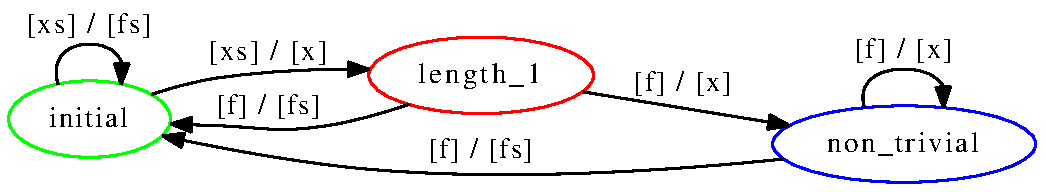
\includegraphics[width=\textwidth]{map_extra_fa.pdf}
    \caption{Избыточный конечный автомат Мили для шаблона блока \textit{For-Loop}}
    \label{map:extra_fa}
\end{figure}

Фактически, для любого алгоритма можно построить автомат Мили с не более, чем двумя состояниями: начальным (или тривиальным) и не тривиальным (с отличным от начального внутренним
состоянием) состояниями, однако, в некоторых случаях автомат Мили будет вносить дополнительную неопределенность в поведение блока, не связанную с неопределенностью
входных данных при анализе. Возможен и обратный случай --- в предыдущем примере с шаблоном блока \textit{For-Loop} можно ввести отдельное состояние, отвечающее за списки длины 1.
В данном случае автомат Мили будет выглядеть, как показано на рисунке \ref{map:extra_fa}, дополнительное состояние именуется \textit{length\_1}. Это дополнительное состояние, конечно,
несет новую информацию о текущем состоянии блока, но она абсолютно бесполезно для анализа схемы потока данных.

\subsection{Эквивалентность траекторий запуска потока данных \textbf{***Need review***}}
  Рассмотрим подробнее правила работы потока данных. В правилах помимо неопределенностей в выборе вариантов поведения, присутствует множество $\phi^t$, задаваемое извне.
  Фактически это множество определяет время работы каждого запущенного блока и введено для возможности описания любой возможной конфигурации времен работы алгоритмов блоков.
  Однако при анализе потока данных эти времена неизвестны и здесь не будут рассматриваться их оценки. Для анализа большее значения играет не сами времена работы блоков, а
  зависимости типа "запуск блока $A$ был вызван завершением работы блоков $B_1, B_2, \dots, B_l$".
  В дальнейшем, для выяснения всевозможных поведений потока данных в терминах этих зависимостей,
  мы будем эмулировать запуск потока данных по правилам \eqref{freetofree}-\eqref{newstate}, и, в частности, положим времена работы всех блоков равными единице.
  Модельное время в данном случае отражает лишь один из возможных случаев запуска потока данных и служит только для удобства понимания.
  Вначале определим понятие траектории запуска потока данных и введем на множестве траекторий запуска отношение эквивалентности.
  
  \begin{defen}
    Траекторию запуска потока данных $\Lambda = \{\Lambda^t\}_{t=0}^{\infty}$ мы определим как семейство всех множеств упомянутых в
    правилах работы потока данных \eqref{freetofree}-\eqref{newstate} и описывающих состояние потока данных,
    то есть $\Lambda^t = (\omega^t, \{\omega^t_{I, v} \vert v \in B_c\}, \{\omega^t_{O, v} \vert v \in B_c\}, \pi^t, s^t, \xi^t, \theta^t, \chi^t$.
  \end{defen}
  
  Введем также определения конечной и успешной траекторий и времени работы потока данных на этой траектории.
  \begin{defen}
    Траектория запуска потока данных $\Lambda = \{\Lambda^t\}_{t=0}^{\infty}$ называется конечной, если
    $\exists T_{end}: \forall t \geq T_{end}: \theta^t = \varnothing$. Минимальное $T_{end}$ называется временем работы потока данных.
    \label{def:trajectory_finite}
  \end{defen}
  
  \begin{defen}
    Траектория запуска потока данных $\Lambda = \{\Lambda^t\}_{t=0}^{\infty}$ называется успешной, если
    $\exists T_{end}: \forall t \geq T_{end} : \xi^t = B_c \wedge \omega^t = \varnothing$.
    \label{def:trajectory_success}
  \end{defen}
  
  Понятно, что минимальные $T_{end}$ из определений \ref{def:trajectory_finite} и \ref{def:trajectory_success} совпадают (если оба существуют), и более того, равны
  (с точностью до времени работы блока $\stock$, которое, для удобства положим равным $0$) $T_{end}$ в \eqref{end_of_workflow}, так как при отсутствии работающих
  блоков фронт активной волны $\omega^t$ не может меняться (в силу правила работы потока данных \eqref{newomega}),
  а значит правило \eqref{blocktofree} не может быть выполнено для заблокированных блоков, так как оно полностью определяется фронтом активной волны.
  В дальнейшем мы будем предполагать, что все траектории рассматриваемого потока данных являются конечными.
  
  Множества $\pi^t_v$, $\omega^t_{I, v}$ и $\omega^t_{O, v}$ полностью описывают отношение эквивалентности между траекториями.
  \begin{defen}
    Для каждой конечной траектории запуска множества $\pi^t_v$, $I^t_v$ пораждают граф причинности $G = (S, E)$.
    Для каждого блока пронумеруем все времена его запуска $t^n_v$. Тогда $G$ можно определить как:
    \begin{itemize}
      \item $S = \{ (v, n, \pi^{t^n_v}_v) \}$,\\
      \item из $s_1 = (v, \cdot, \pi_1)$ в $s_2 = (v, \cdot, \pi_2)$ есть ребро тогда и только тогда,
      когда часть поглощенной $\omega^t_{I, v}$ в результате перехода $\pi_2$ была испушена в результате перехода $\pi_1$;
      при этом ребро дополнительно помечается множеством соответствующих входных портов блока $v$.
    \end{itemize}
  \end{defen}
  
  Отображение $G_{\Lambda} = G(\Lambda)$ индуцирует классы эквивалентности траекторий запуска потока данных,
  иными словами $\Lambda_1 \sim \Lambda_2 \Leftrightarrow G(\Lambda_1) = G(\Lambda_2)$.
  Отметим, что данное отношение эквивалентности имеет смысл только для успешных траекторий, так как в нем не учитываются остаточные активные волны и заблокированные блоки.
  Наличие неуспешных траекторий потока данных мы будем рассматривать как ошибку проектирования схемы потока данных. Отметим, что это правило полностью соответствует практике.
  
  Каждый граф причинности качественно описывает запуск потока данных.
  
  \begin{example}
  \label{map_example}
  Рассмотрим один показательный пример нахождения графов причинности для потока данных, содержащего цикл (схема потока данных изображена на рисунке \ref{example:composite}).
  Для простоты, будем считать, что автомат Мили блока $f$ состоит из одного состояния и одного перехода $\pi_f = (\initial, \{x\}, \{f\}, \initial)$.  
  Наличие ребра из $s_1$ в $s_2$ в графе причинности будем обозначать как $s_1 \leadsto s_2$.
  
  Начальная вершина всех графов причинности --- $s_0 = (\source, 0, \pi_{\source})$. Далее возможны варианты: либо начальная вершина вызовет переход
  $\pi_{\map, 1} = (\initial, \{xs\}, \{fs\}, \initial)$ (то есть переход по пустому списку данных), либо $\pi_{\map, 2} = (\initial, \{xs\}, \{x\}, \nontrivial)$.
  Последний в свою очередь вызовет переход $\pi_f$, который, в свою очередь, может вызвать переходы
  $\pi_{\map, 3} = (\nontrivial, \{f\}, \{x\}, \nontrivial)$ и $\pi_{\map, 4} = (\nontrivial, \{f\}, \{xs\}, \initial)$, и так далее.
  Конечная вершина графа --- $s_{end} = (\stock, T_end, \pi_{\stock})$.
  Получаем семейство графов причинности:
  \begin{eqnarray*}
    s_0 & \leadsto & (\map, t_1, \pi_{\map, 1}) \leadsto s_{end}, \\
    s_0 & \leadsto & (\map, t_1, \pi_{\map, 2}) \leadsto (f, t_2, \pi_f) \leadsto (\map, t_3, \pi_{\map, 4}) \leadsto s_{end}, \\
    s_0 & \leadsto & (\map, t_1, \pi_{\map, 2}) \leadsto (f, t_2, \pi_f) \leadsto (\map, t_3, \pi_{\map, 3}) \leadsto \\
    & \leadsto & (f, t_4, \pi_f) \leadsto \dots \leadsto (\map, t_n, \pi_{\map, 4}) \leadsto s_{end}
  \end{eqnarray*}
  
  \end{example}
  
  Этот пример демонстрирует необходимость следующего предположения:
  \textit{будем считать, что любая циклическая зависимость конечна (то есть не будем рассматривать не конечные траектории, возникающие из-за этих зависимостей)}.
  
\subsection{Неопределенности в запуске потока данных \textbf{***Need review***}}
  Как было упомянуто выше, в анализе схемы потока данных неизбежно возникают два рода неопределенностей: первый вызван отсутствием знания входных данных при анализе схемы,
  неопределенности второго рода связанны с самой схемой потока данных, которая может допускать такие неоднозначности как, например, несколько вариантов поглощения данных.
  Неоднозначности первого рода неизбежны, и поэтому следует обрабатывать все варианты порожденные ими.
  Все эти неоднозначности второго рода возникают как следствие состояний гонки (race condition), которых традиционно стараются избегать,
  так как результат выполнения всего потока данных становиться зависим от времен работы блоков, которые, в свою очередь, могут зависеть от данных и
  параметров вычислительных узлов, что говорит скорее о неправильном построении схемы потока данных.
  
  Сформулируем теперь критерии неопределенностей первого и второго рода.
  
  Любые неопределенности связаны с правилом запуска потока данных \eqref{freetostart} --- правило запуска блока, что видно из правил работы потока данных, так как,
  только это правило содержит включения, вместо строгих равенств.
  \begin{defen}
    Будем говорить, что состояние $s$ автомата Мили $\FA_v = (S_v, \cdot, \cdot, \cdot, E_v)$ блока $v$ допускает неопределенность первого рода, тогда и только тогда, когда:
    $\exists I_v: \lvert \{e \in E_v \vert e = (s, I_v, \cdot, \cdot) \} \rvert > 1$, или иными словами, существует набор входных портов $I_v$, такой что, из состояния $s$ возможны
    несколько переходов по входным портам $I_v$.
  \end{defen}
  
  Например, в автомате Мили шаблона блока \textit{For-Loop} (рисунок \ref{map:fa}) каждое состояние допускает неопределенность первого рода.
  Причины возникновения этих неопределенностей были описанны выше.
 
  \begin{defen}
    Блок $v \in B_c$ в состоянии $\Lambda^t$ траектории запуска потока данных на шаге $t$ допускает неопределенность второго рода, если:
    $\lvert \omega^t_{I, v} \rvert > 1$, где $\omega^t_{I, v}$ определена в правиле \eqref{freetostart} и содержиться в кортеже $\Lambda^t$.
  \end{defen}
  
  \begin{defen}
    \textbf{Корректным потоком данных} будем называть поток данных, любая возможная траектория которого не допускает неопределенностей второго рода.
  \end{defen}
  
  Заметим, что по автомату Мили можно сразу предсказать возможные неопределенности второго рода, например, если автомат Мили содержит переходы
  $\pi = (s, I, \cdot, \cdot)$ и $\pi' = (s, I', \cdot, \cdot)$,
  где $I \subseteq I'$: в этом случае переход по $\pi'$ автоматически означает неопределенность второго рода,
  соответственно, наличие таких переходов автоматически означает неправильность построения автомата Мили или алгоритма блока.
  
  Введем вспомогательное определение набора последовательностей времен работы блоков.
  \begin{defen}
    Зафиксируем набор последовательностей времен работы $\tau = \{\{\tau^n_v\}^{\infty}_{n = 0} \vert v \in B_c\}$.
    Траектория $\Lambda$ согласуется с набором последовательностей времен запуска, если время работы $n$-го запуска блока $v$ $t^n_v = \tau^n_v$.
  \end{defen}
  
  \begin{theorem}
    \label{indeterminacy_theorem}
    В работе потока данных не существует других неопределенностей, кроме неопределенностей первого и второго рода, то есть,
    если зафиксировать набор последовательностей времен работы блоков $\tau$, то любое ветвление префиксного дерева траекторий, согласующихся с $\tau$,
    описывается только неопределенностями первого и второго рода.
  \end{theorem}
  \begin{proof}
    Доказательство напрямую следует из факта, что любые различия в траекториях запуска потока данных при фиксированных временах работы блоков определяются
    правилом \eqref{freetostart} работы потока данных.
  \end{proof}
  
  Среди неопределенностей второго рода следует выделить важный случай, уже упоминавшийся выше --- состояние гонки.
  
  \begin{defen}
    Поток данных допускает состояние гонки, если существует некая последовательность времен запуска $\tau$ и класс эквивалентности $\mathbb{K}$
    траекторий запуска потока данных, такие что траектории удовлетворяющие $\tau$ не лежат в классе $\mathbb{K}$.
  \end{defen}
  
  Поясним это определение. Из определения сразу же следует, что в отсутствии состояния гонки, каждый класс эквивалентности для любого набора последовательностей
  времен запуска содержит траекторию, согласующуюся с ней, что означает то,
  что результат не зависит от времен работы блоков (что соответствует классическим определениям).
  
\subsection{Волновой алгоритм}  
  Решение задачи нахождения классов эквивалентности траекторий запуска позволяет существенно упростить анализ потока данных, так как
  переход к графам причинности позволяет избавиться от модельного времени для корректных потоков данных.
  
  Однако, даже для корректного потока данных, классов эквивалентности может быть бесконечное количество. Это утверждение было проиллюстрированно в примере \ref{map_example}.
  Одним из возможных решений этой проблемы --- нахождение циклов и их замена на соответствующий составной блок. Однако, это не всегда удается, например,
  из-за того, что 'тело' цикла может иметь связи с самим блоком цикла. Однако, если замена циклов удалась, то поток данных будет преобразован к ацикличному графу,
  работу которого заметно проще анализировать. В данной работе рассматривается иной метод избавления от циклических зависимостей путем неявного построения
  'внутреннего' автомата Мили, который можно известными из теории синтаксического анализа алгоритмами преобразовать к 'внешнему' автомату Мили, который
  можно использовать для представления потока данных как единого составного блока в иерархическом потоке данных.

\subsubsection{Волновой алгоритм для ацикличного корректного потока данных}
  Вначале рассмотрим самый простой случай --- анализ ацикличного корректного потока потока данных. Задача волнового алгоритма
  перебрать все возможные классы эквивалентности траекторий запуска потока данных, которую он выполняет путем перебора по единичным траекториям из каждого класса.
  Вначале докажем один простой факт, из которого вместе с \ref{indeterminacy_theorem} частично следует коррекность алгоритма \ref{simple_wave_alg}.
  
  \begin{theorem}
    \label{finite_theorem}
    Классы эквивалентности траекторий запуска ацикличного корректного потока данных образуют конечное множество.
  \end{theorem}
  \begin{proof}
    Докажем от противного. Если множество классов эквивалентности не конечно, то для любого $N \in \mathbb{N}$ существует блок в этом потоке данных и граф причинности,
    в котором этот блок был запущен более $N$ раз, так как количество блоков в любом потоке данных конечно. Так как поток данных по условию ацикличен, то
    любая волна данных не может вернуться к входным портам порадившим ее блокам, а в силу конечности начальной волны любой блок будет запущен
    заведомо не более, чем $\lvert E_c \rvert$ раз, где $E_c$ --- множество ребер рассматриваемого потока данных. Противоречие.
  \end{proof}
  
  Рассмотрим теперь подробно работу алгоритма \ref{simple_wave_alg}. В строках 2-13 происходит формирование множества наборов возможных переходов.
  В эти наборы попадают переходы, которые могут запуститься ($\pi \in \FA(s_v, I_v(\omega))$) и успешно излучить данные ($\zeta(\omega, \sigma)$).
  В строках 14-20 записано условие окончание работы потока данных в соответствии с определением \ref{def:trajectory_success}. Заметим, что выполнение
  строки 18 означает, что траектория не является успешной, так как существует остаточная активная волна, которая не способна запустить ни одного блока.
  Выполнение строки 16 означает, что на вход подан завершившийся поток данных --- функция возвращает граф уже построенный граф причинности.
  Далее в строках 22-41 происходить перебор всевозможных сочетаний переходов блоков, функция \text{Samples} (код которой не представляет интереса) должна вернуть
  эти всевозможние сочетания. В строках 34-37 происходит дополнения неполного графа причинности для текущего случая.
  Заметим, что выполнение строки 32 означает более одного варианта поглощения, что является неопределенностью второго рода и рассматривается как ошибка.
  Докажем корректность алгоритма.
  
  \begin{theorem}
    Функция \textbf{Wave} из алгоритма \ref{simple_wave_alg} при запуске $\text{Wave}(c, (S_0, \omega_0), (\varnothing, \varnothing))$ на корректном
    ацикличном потоке данных $c$ возвращает множество всех возможных графов причинности.
  \end{theorem}
  \begin{proof}
    Для даказательства внимательно рассматрим возращаемые значения алгоритма. Вначале рассмотрим случай незавершенного состояния
    потока данных (то есть допускающего запуск блоков).
    Рассмотрим строки 14-20. Так как по условию поток данных корректный, а значит в частности не содержит состояний гонки, то запуск блока не в момент
    выполнения условия запуска \ref{freetostart}, а в момент выполнения условий запуска и узлучения эквивалентен изменению времени работы блока до момента
    выполнения условия узлучения, и не влияет на граф причинности обрабатываемых классов эквивалентности. А значит перебор возможных переходов из данного состояния
    происходит корректно.
    В строке 40 происходит сбор результатов стартов алгоритма из новых начальных условий с дополненными графами причинности.
    В силу теоремы \ref{finite_theorem} и вышесказанного все рекурсивные вызовы функции закончатся на строке 16, вернув один из графов причинности
    завершенного потока данных.
    Так как любой поток данных стартует из одного состояния ($(S_0, \omega_0)$) и на каждом шаге рассматриваются все возможные варианты запуска блоков
    (также можно показать, что все графы причинности различны), то вызов функции с начальными условиями вернет множество всех графов причиности, перебрав
    тем самым все классы эквивалентности.
  \end{proof}
  
  \begin{algorithm}
    \caption{Волновой алгоритм для случая ацикличного корректного потока данных}
    \label{simple_wave_alg}
    \begin{algorithmic}[1]    
      \Function{Wave}{$c = (B_c, E_c), S_c = (S_B, \omega), g_R = (V, E)$}
        \State $\Pi \leftarrow \text{empty}$
        \ForAll{$v \in B_c, v \neq \stock$}
          \State $\Pi_v \leftarrow \varnothing$
          \State $s_v \leftarrow \text{StateOfBlock}(S_B, v)$
          \ForAll{$\pi \in \FA_v(s_v, I_v(\omega))$}
            \State $(\sigma, \lambda', q) \leftarrow \pi$
            \If{$\zeta(\omega, \sigma)$}
              \State $\Pi_v \leftarrow \Pi_v \cup \{ \pi \}$
            \EndIf
          \EndFor
          \State $\Pi(v) \leftarrow \Pi_v$
        \EndFor
        
        \Statex
        
        \If{$\Pi = \text{empty}$}
          \If{$\Delta_{I, \stock}(\omega) = \{\omega\}$}
            \State \Return{$\{g_R\}$}
          \Else
            \State \textbf{error} \text{''Ошибка, поток данных не является корректным''}
          \EndIf
        \EndIf
        
        \Statex
        \State $G_R \leftarrow \varnothing$        
        \ForAll{$\pi \in \text{Samples}(c, \Pi)$}
          \State $(V', E') \leftarrow g_R$
          \State $(S_B', \omega') \leftarrow S_c$
          \ForAll{$v \in B_c, v \neq \stock$}
            \If{$\pi(v) \neq \text{empty}$} 
              \State $(\sigma, \lambda', q) \leftarrow \pi(v)$
              \State $\Delta \leftarrow \Delta_{I, v}(v)$
              \If{$\rvert \Delta \rvert = 1$}
                \State $\delta \leftarrow \Delta_1$
              \Else
                \State \textbf{error} {\text{''Ошибка, поток данных не является корректным''}}
              \EndIf
              \State $V' \leftarrow V' \cup \text{Reasons}_c(S_c, \lambda')$
              \State $E' \leftarrow E' \cup \{(r, \pi_r, v, \pi(v)) \vert (r, \pi_r) \in \text{Reasons}_c(\lambda')\}$
              \State $\omega' \leftarrow (\omega' \setminus \delta) \cup \sigma$
              \State $S_B' \leftarrow \text{SetStateOfBlock}(S_B', v, q)$
            \EndIf
          \EndFor
          \State $G_R \leftarrow G_R \cup \text{Wave}(c, (S_B', \omega'), (V', E'))$
        \EndFor
        \Statex
        \State \Return $W$
      \EndFunction
    \end{algorithmic}
  \end{algorithm}

\subsubsection{Волновой алгоритм для корректного потока данных}
  Вернемся теперь к рассмотрению общего случая потоков данных, а именно к потокам с возможным наличием циклов.
  Как уже было показано множество графов причинности потока данных содержащего циклические зависимости может и не быть конечным.
  Заметим, что не всякая циклическая зависимость в графе потока данных эквивалентна циклу в классическом понимании.
  Чтобы убедиться в этом, достаточно изменить поток данных из примера \ref{example:composite},
  убрав ребро $(\nontrivial, \nontrivial)$ из автомата Мили шаблона блока map.
  Поэтому будет говорить, что в потоке данных присутствует цикл, если в нем существует циклическая зависимость, порождающая бесконечное множество графов причинности.
  
  Не сложно убедиться, что подграфы графов причинности, соответствующие циклам (будем называть такой подграф подграфом цикла) в потоке данных, образуют регулярные цепочки.
  Заметим, что для анализа графов причинности достаточно указать графы причинности соответствующие каждой полной итерации.
  Это означает, что существует множество полных итераций --- последовательностей переходов, которые вернут подграф цикла в исходное состояние.
  На обнаружении возвращений в исходное состояние подграфа цикла основана идея модификации волнового алгоритма \ref{simple_wave_alg}.
  Для этого мы будем строить 'внутренний' автомат Мили всего потока данных.
  
  \begin{defen}
    \textbf{Внутренним автоматом Мили} потока данных будем называть граф $\FA_c = (S, E)$, где:
    \begin{itemize}
      \item $S = \Sigma \times 2^{E_c}$ --- множество состояний потока данных (то же, что и в определении потока данных);
      \item $E \subseteq S \times \Pi \times S$ --- множество ребер 'внутреннего' автомата Мили потока данных,
        где $\Pi = \cup_{v \in B_c} \Pi_v$, $\Pi_v$ --- множество переходов автомата Мили блока $v \in B_c$.
    \end{itemize}
  \end{defen}
  
  В отличии от алгоритма \ref{simple_wave_alg} в данном алгоритме мы будем делать по одному запуску блока за итерацию, причем отдавать предпочтение
  испущенным в результате предыдущего запуска данным.
  
  \begin{algorithm}
    \caption{Волновой алгоритм для случая корректного потока данных}
    \label{wave_alg}
    \begin{algorithmic}[1]
      \State $S \leftarrow \varnothing$
      \State $E \leftarrow \varnothing$
      \Function{Wave}{$c = (B_c, E_c), S_B, Q_W$}
         \State $S \leftarrow S \cup \{(S_B, Q_W)\}$
         \State $\omega' \leftarrow \varnothing$
         \State $Q'_W \leftarrow Q_W$
         \While{$\forall v \in B_c : \FA_v(s_v, \omega') = \varnothing \vee \neg \zeta(\sigma, \omega)$}
           \State $\omega' \leftarrow \omega' \cup \{\text{pop}(Q'_W)\}$
         \EndWhile
         \Statex
         \State $v \leftarrow \{v \in B_c \vert \FA_v(s_v, \omega') \neq \varnothing \}_1$
         \State $\Pi \leftarrow \FA(stateOfBlock(S_B, v), I_v(\omega'))$
         \ForAll{$\pi_v \in \Pi$}
           \State $(\sigma, \lambda, q) \leftarrow \pi$
           \State $Q'_W \leftarrow \text{push}(\text{delete}(Q_W, \lambda), \sigma)$
           \State $S'_B \leftarrow SetStateOfBlock(S_B, v, q)$
           \If{$(S'_B, Q'_W) \notin S$}
             \State $S \leftarrow S \cup \{(S'_B, Q'_W)\}$
             \State $E \leftarrow E \cup (S_B, Q_W, \pi_v, S'_B, Q'_W)$
             \State $\text{Wave}(c, S'_B, Q'_W)$
          \Else
             \State $E \leftarrow E \cup (S_B, Q_W, \pi_v, S'_B, Q'_W)$
          \EndIf
         \EndFor
      \EndFunction
    \end{algorithmic}
  \end{algorithm}
  
  Начальный запуск осуществляется как $\text{Wave}(c, S_0, \text{push}(\text{empty\_stack}, \omega_0))$.
  Вспомогательные функции $\text{push}$, $\text{delete}$ и $\text{pop}$ являются стандартными функциями для работы со стеком.
  Заметим, что алгоритм заведомо завершится за конечное количество шагов, так как единственный рекурсивный вызов в строке 19 осуществляется только при отсутствии рассматриваемой
  точки 'внутреннего' автомата Мили в множестве $S$, которое заведомо конечно. Доказательство корректности алгоритма повторяет доказательство
  корректности алгоритма \ref{simple_wave_alg}, с той лишь разницой, что требуется заметить, что одиночный запуск блока за вызов функции $\text{Wave}$ при отсутствии
  состояний гонки (что гарантируется корректностью потока данных) дает корректный автомат Мили.
  
  Поясним теперь необходимость представления активной волны в виде стека. Для этого достаточно рассмотреть поток данных, в котором дополнительная ветка расположена параллельно циклу.
  Так как кортеж $S_B$ содержит состояния всех блоков, то для избежания лишних итераций алгоритма, благодаря стеку, выполнение параллельной ветки 'остановиться' на время выполнения
  рассчета цикла.
  
  Заметим, что полученный 'внутренний' автомат Мили позволяет довольно просто генерировать графы причинности и его можно неформально рассматривать
  как конечный автомат для регулярного 'языка' графов причинности.

\subsection{Анализ графов причинности}
  Переход к графам причинности является главным шагом к анализу запуска потока данных в распределенных средах.
  Фактически граф причинности полностью описывает стратегию запуска потока данных. Все необходимые алгоритмы получения графов причинности по схеме потока данных
  были описаны выше. Здесь мы рассмотрим задачу нахождения наилучшего количества вычислителей для
  запуска потока данных в бесконечной однородной распределенной среде. Для этого достаточно рассмотреть эту задачу для одного графа причинности и объединить результаты.
  
  Заметим, что бессмысленно в общем случае рассматривать какие-либо вероятностные меры на графах причинности. Фактически сопоставление графу причинности
  какой-либо вероятности означает приписывание каждым переходам автоматов Мили блоков вероятностей. Однако практически всегда качественное поведение блоков зависит
  от данных поступивших на вход. Для примера рассмотрим часто встречающийся на практике и уже упомянутый пример потока данных
  (схема потока данных изображена на рисунке \ref{example:composite}). Прежде всего нас будет интересовать вероятности переходов в автомате Мили блока map с шаблоном Loop.
  Сопоставляя вероятности переходам в автомате Мили шаблона Loop, как уже было упомянуто, мы делаем предположение о длине цикла (или длине списка значений).
  \begin{eqnarray*}
    P(\initial \rightarrow \initial) & = & a; \\
    P(\initial \rightarrow \nontrivial) & = & 1 - a; \\
    P(\nontrivial \rightarrow \nontrivial) & = & b; \\
    P(\nontrivial \rightarrow \initial) & = & 1 - b; \\
  \end{eqnarray*}
  \begin{eqnarray*}  
    P(L = 0) & = & P(\initial \rightarrow \initial) = a; \\
    P(L = 1) & = & P(\initial \rightarrow \nontrivial \rightarrow \initial) = \\
             & = & (1 - a) (1 - b); \\
    P(L = 2) & = & (1 - a) b (1 - b); \\
    \cdots & & \\
    P(L = n) & = & (1 - a) b^{n - 1} (1 - b);\\
    \mathbb{E}(L) & = & (1 - a) (1 - b) \sum^{\infty}_{n = 1} n b^{n - 1} = \frac{1 - a}{1 - b} \label{math_expect}
  \end{eqnarray*}
  Количество итераций цикла $L$ напрямую определеяет время работы всего потока данных: $LT_f = \frac{1 - a}{1 - b} T_f$,
  где $T_f = const$ --- время одной итерации (работы блока f) для простоты положим равным константе.
  Из формулы \ref{math_expect} видно, что математическое ожидание количества итераций цикла
  (а значит оценку длины списка в реальных запусках) можно сделать любым, однако количество итераций в реальных задачах может варьироваться в пределах нескольких порядков.
  
  Рассмотрим поток данных и его граф причинности $g_R$. Будем считать, что при запуске поток данных будет вести себя в соответствии с графом причинности $g_R$.
  Пусть также дана распределенная однородная среда бесконечного рамера. Будем считать, что для выполнения одного перехода автомата Мили любого блока требуется однин вычислитель.
  Пусть количество вычислителей, на который выполняется запуск потока данных $N$. Определим задачу оценки оптимального количества ресурсов, как задачу
  нахождения диапазона минимального диапазона $[N_{\min}, N_{\max}]$:
  $$\forall \tau \in \mathbb{K}_{g_R} (\forall N < N_{min} T_{N, \tau} > T_{N_{\min}, \tau}) \wedge (\forall N > N_{max}: T_{N, \tau} = T_{N_{\max}, \tau}),$$
  где $T_{N, \tau}$ --- минимальное время работы потока данных на $N$ вычислителях при наборе времен работы блоков $\tau$.
  Иными словами, задача оценки оптимального количесва ресурсов состоит в поиске таких количеств вычислителей $N_{\min}$ и $N_{\max}$, что
  беря количество вычислителей менее $N_{\min}$, время работы потока данных будет гарантированно меньше, а добавление еще одного вычислителя после $N_{\max}$ не пренесет результата.
  
  Для удобства введем следующее определение.
  \begin{defen}
    Множество $S_{g_R}$ будем называть \textbf{cрезом графа причинности} $g_R = (V, E)$, если
    $S_{g_R} \subseteq V: \forall P \subseteq E \text{--- путь в графе } g_R: \nexists s_1, s_2 \in S_{g_R}: s_1 \xrightarrow{P} s_2$.
  \end{defen}
  Иными словами срез в один срез графа причинности могут входить только переходы, которые могут выполняться одновременно (то есть не зависят друг от друга).
  
  \begin{theorem}
    В любой срез любого графа причинности корректного потока данных не могут входить переходы одного и того же блока.
  \end{theorem}
  \begin{proof}
    Предположим обратное. Заметим, что если $\pi_{1, v}, \pi_{2, v} \in S$, то в потоке данных присутствует состояние гонки. Это напрямую следует из определения
    среза графа причинности, так как переходы $\pi_{1, v}$ и $\pi_{1, v}$ независимы, а значит существуют наборы времен выполнения переходов, такие, что эти
    переходы выполняются в разной последовательности, что и есть определение состояния гонки. Но поток данных по условию корректный. Противоречие.
  \end{proof}
  
  Рассмотрим нахождение $N_{\max}$. Заметим, что $N_{max}$ соответствует максимальной мощности среза графа причинности, так как фактически это максимальное
  количество одновременно выполняемых переходов или максимальное количество вычислителей которое можно задействовать одновременно.
  
  Для определения $N_{\min}$ потребуется ввести дополнительные определения.
  \begin{defen}
    Будем говорить, что срез графа причинности $g_R = (V, E)$ $S_2$ следует из среза $S_1$, если:
    $$S_1 \leadsto S_2 \Leftrightarrow S_1 \neq S_2 \wedge \{(e_1, e_2) \vert e_1 \in S_1, e_2 \in S_2\} \subseteq (V \cup \{(e, e) \vert e \in S_1 \cap S_2\})$$
  \end{defen}
  Иными словами $S_1 \leadsto S_2$ означает, что вершины $S_1$ и $S_2$ находяться на расстоянии не более 1 шага и $S_1 \neq S_2$.
  
  \begin{defen}
    \textbf{Эволюция графа причинности} --- последовательность $\Delta = \{S^j\}^{J}_{j = 0}$, где $S^0 = \{(\pi_{\source}, 1)\}$,
    $S^J = \{(\pi_{\stock}, 1)\}$ и $\forall J \geq j > 1: S^{j - 1} \leadsto S^j$.
  \end{defen}
  
  \begin{theorem}
    Любой эволюции $\Delta = \{S^j\}^J_{j = 0}$ графа причинности соотвествует как минимум один набор времен работы блоков $\tau$, при котором
    множества работающих блоков запуска потока данных $\forall t \in [0, T_{\text{end}}]: \theta^t = S^t$.
  \end{theorem}
  \begin{proof}
    Построим требуемый набор времен работы блоков. Для этого достаточно положить время $n$-го перехода $\pi_v$ равным
    $\max \{j_1 - j_2: \forall j \in [j_1, j_2]: (\pi_v, n) \in S_j\}$. Нетрудно показать, что такие времена работы блоков удовлетворяют условию теоремы.
  \end{proof}
  
  Несложно убедиться используя доказанную выше теорему, что $$N_{\min} = \min_{\Delta} \max_{S^j \in \Delta} \lvert S^j \rvert$$
  Для единообразия переформулируем равенство для $N_{\max}$:
  $$N_{\max} = \max_{S} \lvert S \rvert = \max_{\Delta} \max_{S^j \in \Delta} \lvert S^j \rvert$$
  
  Для поиска оценок $N_{\max}$ и $N_{\min}$ существуют разнообразные модификации алгоритма HELF \textbf{[???]},
  позволяющие вычислять как точные, так и оценочные значения описанных величин.
  
 \subsubsection{Динамическая корректировка зарезервированных ресурсов}
   Для каждого графа причинности существуют две оценки $N_{\max}$ и $N_{\min}$ количества необходимых вычислителей.
   Основной проблемой является то, что точный граф причинности текущего запуска потока данных может быть неизвестен вплоть до конца работы.
   Однако можно заметить, что графы причинности образуют префиксное дерево (это видно уже из волнового алгоритма), поэтому возможно
   динамическое (runtime) уточнение множества возможных графов причинности. Заметим, что проверка, является ли граф причинности подграфом другого, осуществляется
   за линейное время, так как между вершинами графов причинности существует единственное соответствие. Построение же префиксного дерева неявно осуществляется во время работы
   волнового алгоритма.
   
   Итак, пусть дано префиксное графов причинности. Сопоставим каждой вершине $g$ этого дерева четыре величины $\hat{N}_{\min, \min}(e)$, $\hat{N}_{\min, \max}(e)$,
   $\hat{N}_{\max, \min}(e)$, $\hat{N}_{\max, \max}(e)$: соотвественно максимум/минимум максимумов/минимумов постфиксов графов причинности с префиксом $g$.
   Заметим, что некоторые модификации алгоритма HELF позволяют дешево перевычислить оценки соотвествующих величин при достроении графа причинности.
   Каждая оценка несет свой смысл, например, $N_{\max, \max}$ --- максимальное количество вычислителей, одновременно задействованных в 'худшем' случае.
   
   Пример динамического изменения оценок приведен на рисунке \ref{example2}.
   
   \begin{figure}[H]
  \centering

  \begin{subfigure}[b]{\textwidth}
    \centering
    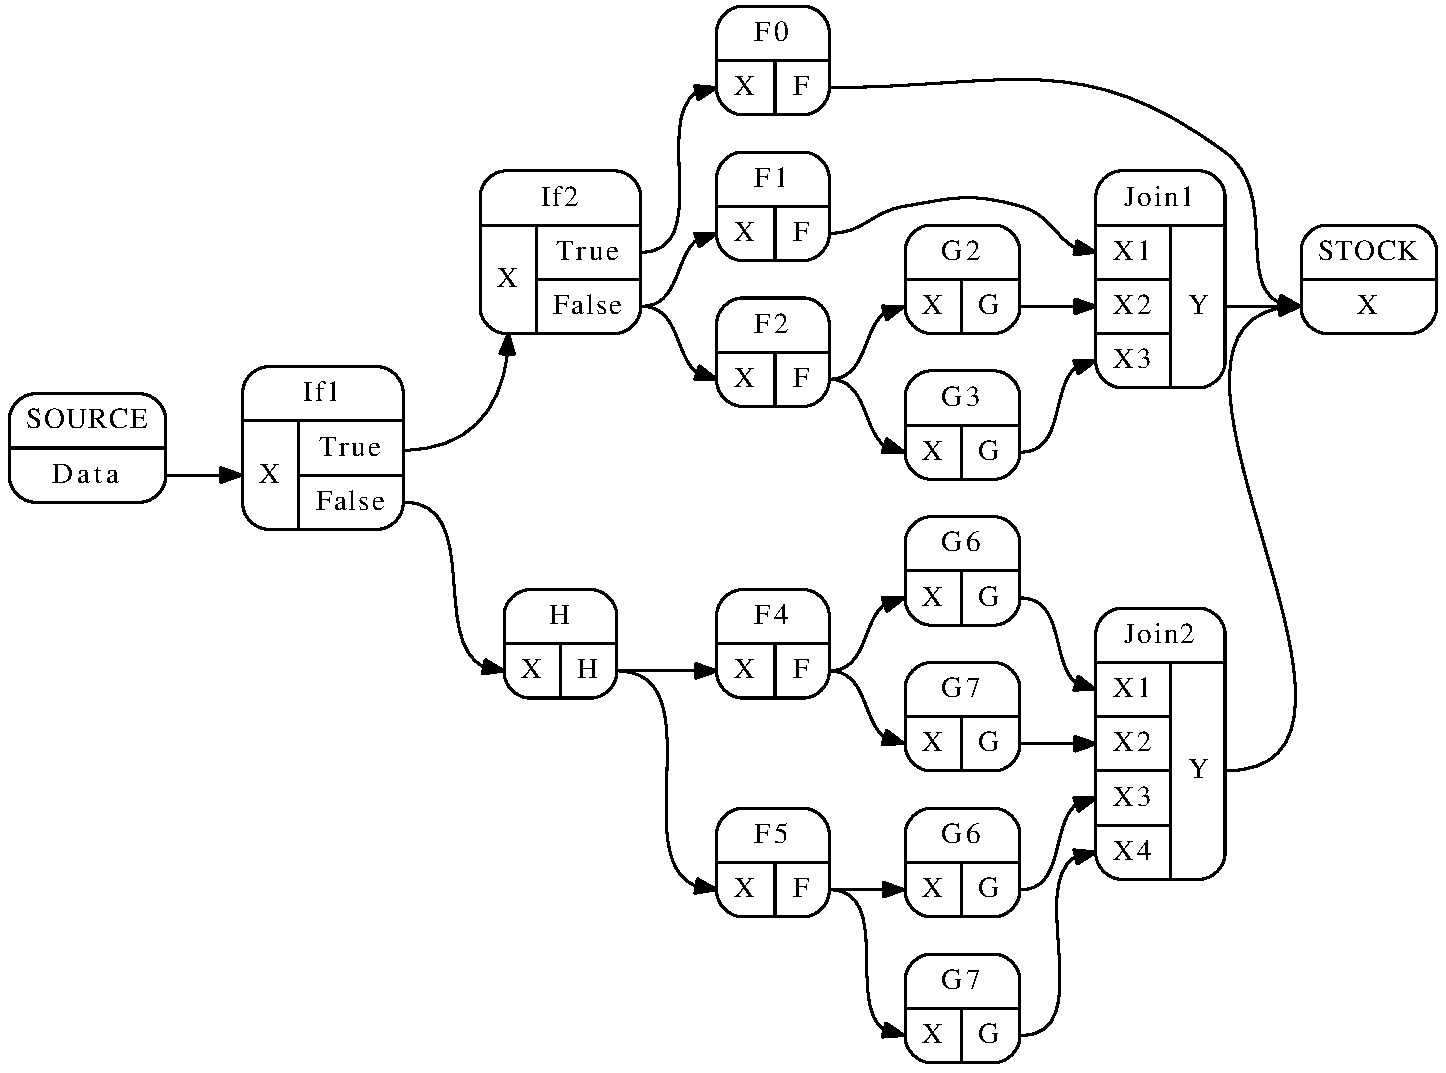
\includegraphics[width=\textwidth]{example2.pdf}
    \caption{Пример схемы шаблона потока данных}
    \label{map:connection}
  \end{subfigure}
  ~
  \begin{subfigure}[b]{\textwidth}
    \centering
    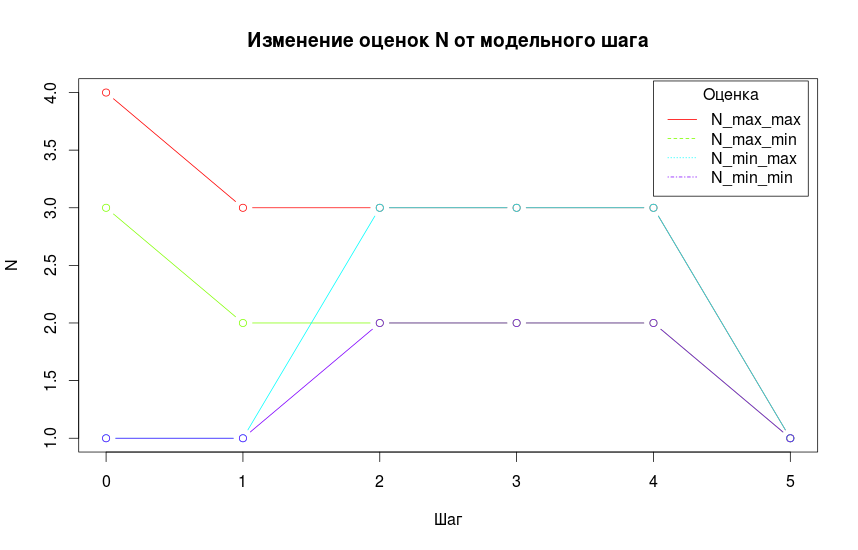
\includegraphics[width=\textwidth]{Rplot01}
    \caption{Поведение оценок в зависимости от шага по префексному дереву графов причинности
             в случае переходов If1 по ветке True (шаг 1), If2 по ветке False (шаг 2)}
    \label{map:fa}
  \end{subfigure}
  
  \caption{Пример динамического изменения оценок числа $N$}
  \label{example2}
  \end{figure}
  
\subsection{Поиск неопределенностей второго рода}
  

\section{Заключение}

\end{document}